\documentclass[a4paper]{article}

\usepackage{ctex}
\usepackage[utf8]{inputenc}
\usepackage[margin=1in]{geometry}
\usepackage[T1]{fontenc}
\usepackage{textcomp}
\usepackage[dutch]{babel}
\usepackage{amsmath, amssymb}
\usepackage{hyperref}
\usepackage{titlesec}
\hypersetup{
  colorlinks=true,
  linkcolor=blue,
  filecolor=magenta,
  urlcolor=cyan,
  pdfauthor={Matrix},
  pdftitle={},
  pdfkeywords={},
  pdfsubject={},
  pdfcreator={Emacs 27.2 (Org mode 9.4.4)},
  pdflang={English}
  }
\urlstyle{same}


% figure support
\usepackage{import}
\usepackage{pdfpages}
\usepackage{transparent}
\usepackage{xcolor}
\newcommand{\incfig}[2][1]{%
    \def\svgwidth{#1\columnwidth}
    \import{./figures/}{#2.pdf_tex}
}

\begin{document}
\urldef\fitlmurl\url{https://www.mathworks.com/help/stats/fitlm_zh_CN.html#bt0ck7o-4}
\section{环形水槽参数率定}
环形水槽的控制系统输入频率$x$与环形水槽的转速$y$之间存在\textbf{线性关系}:$y=a \cdot x+b$,利用以下数据借助MATLAB的\texttt{fitlm}\footnote{fitlm: \fitlmurl}函数计算这一线性关系表达式系数:$a$ 和$b$,并得到剪力环转速$\omega_t = 1.5 \rm rpm $, $3.0\rm  rpm $和$4.5\rm rpm $对应的控制系统输入频率。

\begin{table}[htbp]
	\centering
\begin{tabular}{ccc}
\hline
\multicolumn{1}{l}{软件输入频率$x$} & \multicolumn{1}{l}{剪力环旋转圈数} & \multicolumn{1}{l}{用时(min)} \\ \hline
20                         & 3                           & 2.763                       \\
40                         & 3                           & 1.366833333                 \\
60                         & 3                           & 0.906166667                 \\
80                         & 5                           & 1.137                       \\
100                        & 6                           & 1.089                       \\ \hline
\end{tabular}
\end{table}

\begin{table}[htbp]
	\centering
\begin{tabular}{ccc}
\hline
\multicolumn{1}{l}{软件输入频率$x$} & \multicolumn{1}{l}{环形水槽旋转圈数} & \multicolumn{1}{l}{用时(min)} \\ \hline
-20                        & 3                           & 4.313166667                 \\
-40                        & 4                           & 2.929833333                 \\
-60                        & 4                           & 1.963166667                 \\
-80                        & 5                           & 1.849333333                 \\
-100                       & 5                           & 1.485                       \\ \hline
\end{tabular}
\end{table}

\section{PIV采样频率}
考虑环形水槽中轴线的线速度$V$作为流体的最大速度,其中水槽内直径$D_i = 3.0 \rm m $ ,外直径$D_o=3.6\rm m$。当查询窗口为$32 \mathrm{pix} \times 32 \mathrm{pix}$时,针对剪力环转速$\omega_t = 1.5 \rm rpm $, $3.0 \rm rpm $和$4.5 \rm rpm $三种工况,计算流体的最大速度$V$;并进一步计算高速相机的最低采样频率\footnote{最低采样频率保证最大速度的流体在拍摄的相邻两张照片中位移不超过查询窗口的一半尺寸,即$16 \rm pix$。}(frame per second, fps),假定比例尺$\mathrm{scale} = 7\times 10^{-5} \rm {m}/{pix}$。

\section{burst mode (long-term continuous shooting) 采样参数}
图\ref{fig:Picture1-png}展示了参数为:采样频率$500\rm fps$ ,burst period $700\rm \mu s$,burst count  $2$,曝光时间$200 \rm \mu s$的相机burst mode拍摄触发模式。请问,采用burst mode拍摄模式得到的相机照片序列进行PIV计算时,用于计算瞬时速度的相邻两张照片时间间隔$\Delta t$ 应该取 burst period $700\rm \mu s$ 还是采样频率$500 \rm fps$对应的$2000 \rm \mu s$?

\begin{itemize}
	\item Burst Count - Burst Count sets the number of frames in a burst, (a value of zero disables burst mode completely).
	\item Burst Period - Burst Period sets the interval between two frames in a burst, in microseconds.
\end{itemize}
\begin{figure}[htpb]
	\centering
	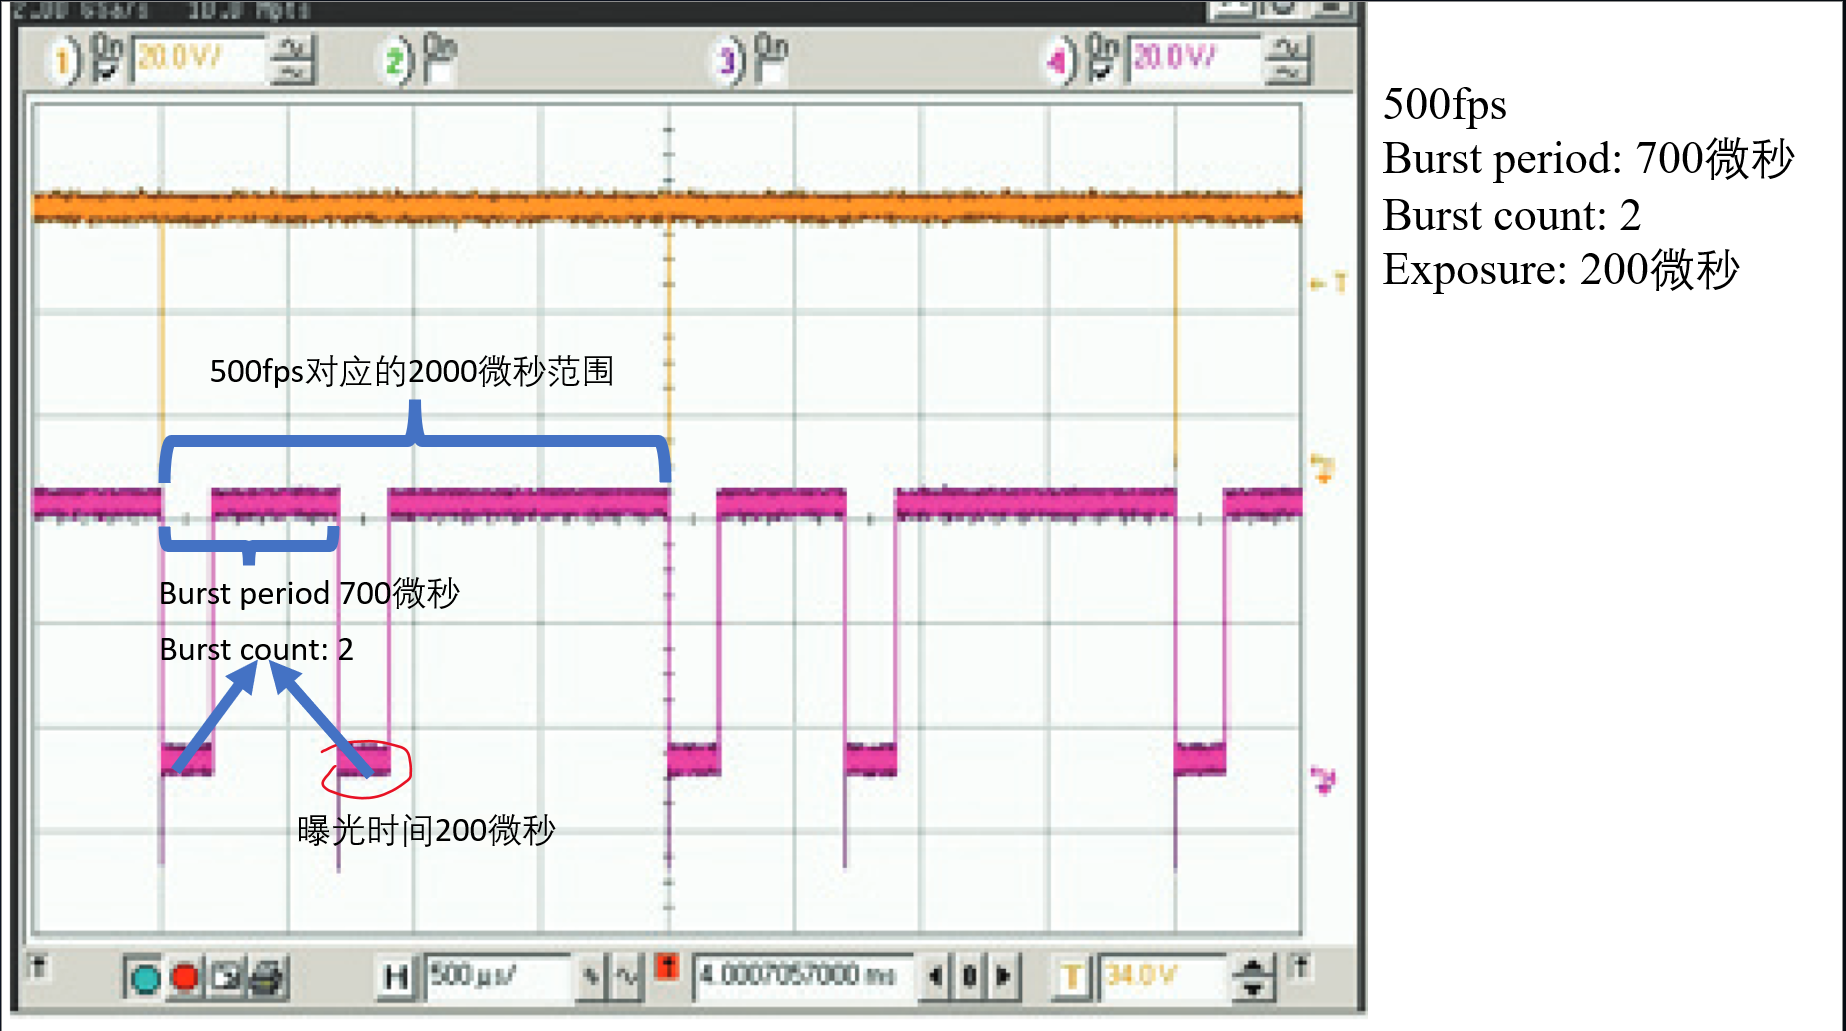
\includegraphics[width=0.8\textwidth]{Picture1.png}
	\caption{burst mode拍摄触发模式}
	\label{fig:Picture1-png}
\end{figure}
\end{document}
